\chapter{Modeling the economically utilisable wood in the crown of European beech trees}
\label{chap:beech_crowns}
{\large Kai Husmann$^1$ - Bernhard M�hring$^1$}\\

\vspace{3cm}
\noindent
$^1$Department of Forest Economics and Forest Management,\\ University of G�ttingen, B�sgenweg 3, 37077 G�ttingen, Germany \\

\vspace{\fill}
\noindent
Published in:\\
Forest Policy and Economics.\\(DOI: X)


\cleardoublepage
%%%%%%%%%%%%%%
%% Abstract %%
%%%%%%%%%%%%%%
\section*{Abstract}
\label{chap:beech_crowns:Abstract}
Abstract.

\subsection*{Keywords}
Keywords


%%%%%%%%%%%%%%%%%%
%% Introduction %%
%%%%%%%%%%%%%%%%%%
\section{Introduction}
\label{sec:beech_crowns:Introduction}
Introduction.

\begin{figure}
\center
  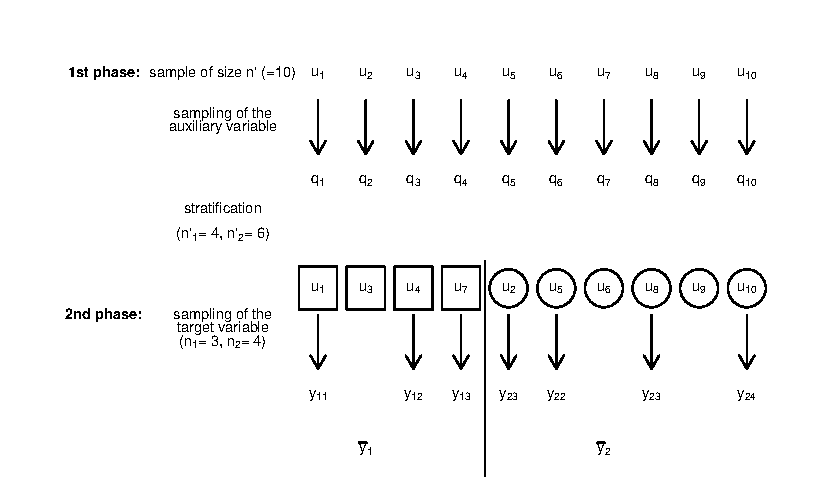
\includegraphics{Grafiken/beech_crowns/example.pdf}
\caption{Example 1.}
\label{fig:beech_crowns:ex1}
\end{figure}

Further text.

%%%%%%%%%%%%%%%%%%%%%%%%%%%
%% Materials and Methods %%
%%%%%%%%%%%%%%%%%%%%%%%%%%%
\section{Materials and Methods}
\label{sec:beech_crowns:methods}

Examples can be found in \citet{Mandallaz_2008} see also \citep{Gregoire_2008,Mandallaz_2008}.

%%-------------------------------------%%
%% Data sampling and sample processing %%
%%-------------------------------------%%
\subsection{Selection of trees}
\label{subsec:beech_crowns:methods:tree_selection}

Data

%%--------------------%%
%% Selection of disks %%
%%--------------------%%
\subsection{Selection of disks}
\label{subsec:beech_crowns:methods:disk_selection}

Disk selection.

%%-----------------------%%
%% Selection of branches %%
%%-----------------------%%
\subsection{Selection of branches}
\label{subsec:beech_crowns:methods:branch_selection}

Branch selection.

%%--------------------------------------------------------%%
%% Estimation of wood volume in the stem and in the crown %%
%%--------------------------------------------------------%%
\subsection{Estimation of wood volume in the stem and in the crown}
\label{subsec:beech_crowns:methods:crown_vol_est}

crown vol est.

%%----------------------------------------------%%
%% Economically viable wood volume in the crown %%
%%----------------------------------------------%%
\subsection{Economically viable wood volume in the crown}
\label{subsec:beech_crowns:methods:viable}

Viable.

%%++++++++++++++++++++++++++++%%
%% Crown type differentiation %%
%%++++++++++++++++++++++++++++%%
\subsubsection{Crown type differentiation}
\label{subsubsec:beech_crowns:methods:viable:crown_types}

Crown types.

%%++++++++++++++++++++++++++++++++++++++++++++++++++++++++++++%%
%% Modelling the economically viable wood volume in the crown %%
%%++++++++++++++++++++++++++++++++++++++++++++++++++++++++++++%%
\subsubsection{Modelling the economically viable wood volume in the crown}
\label{subsubsec:beech_crowns:methods:viable:econ_viable}

Modelling the economically viable wood volume in the crown.

%%--------------------------%%
%% Allometric relationships %%
%%--------------------------%%
\subsection{SAllometric relationships}
\label{subsec:beech_crowns:methods:allo}

Allometric relationships.


%%%%%%%%%%%%%
%% Results %%
%%%%%%%%%%%%%
\section{Results}
\label{sec:beech_crowns:results}

%%------------------------------%%
%% Estimation of bark thickness %%
%%------------------------------%%
\subsection{Estimation of bark thickness}
\label{subsec:beech_crowns:results:bark}

Estimation of bark thickness.

%%----------------------------------------------%%
%% Economically viable wood volume in the crown %%
%%----------------------------------------------%%
\subsection{Economically viable wood volume in the crown}
\label{subsec:beech_crowns:results:viable}

Viable.

%%++++++++++++++++++++++++++++%%
%% Crown type differentiation %%
%%++++++++++++++++++++++++++++%%
\subsubsection{Crown type differentiation}
\label{subsubsec:beech_crowns:results:viable:crown_types}

Crown types.

%%++++++++++++++++++++++++++++++++++++++++++++++++++++++++++++%%
%% Modelling the economically viable wood volume in the crown %%
%%++++++++++++++++++++++++++++++++++++++++++++++++++++++++++++%%
\subsubsection{Modelling the economically viable wood volume in the crown}
\label{subsubsec:beech_crowns:results:viable:econ_viable}

Modelling the economically viable wood volume in the crown.

%%--------------------------%%
%% Allometric relationships %%
%%--------------------------%%
\subsection{SAllometric relationships}
\label{subsec:beech_crowns:results:allo}

Allometric relationships.


%%%%%%%%%%%%%%%%
%% Discussion %%
%%%%%%%%%%%%%%%%
\section{Discussion}
\label{sec:beech_crowns:discussion}

%%------------------------------%%
%% Estimation of bark thickness %%
%%------------------------------%%
\subsection{Estimation of bark thickness}
\label{subsec:beech_crowns:discussion:bark}

Estimation of bark thickness.

%%----------------------------------------------%%
%% Economically viable wood volume in the crown %%
%%----------------------------------------------%%
\subsection{Economically viable wood volume in the crown}
\label{subsec:beech_crowns:discussion:viable}

Viable.

%%++++++++++++++++++++++++++++%%
%% Crown type differentiation %%
%%++++++++++++++++++++++++++++%%
\subsubsection{Crown type differentiation}
\label{subsubsec:beech_crowns:discussion:viable:crown_types}

Crown types.

%%++++++++++++++++++++++++++++++++++++++++++++++++++++++++++++%%
%% Modelling the economically viable wood volume in the crown %%
%%++++++++++++++++++++++++++++++++++++++++++++++++++++++++++++%%
\subsubsection{Modelling the economically viable wood volume in the crown}
\label{subsubsec:beech_crowns:discussion:viable:econ_viable}

Modelling the economically viable wood volume in the crown.

%%--------------------------%%
%% Allometric relationships %%
%%--------------------------%%
\subsection{Allometric relationships}
\label{subsec:beech_crowns:discussion:allo}

Allometric relationships.

%%%%%%%%%%%%%%%%%%%%%%%%%%%%%
%% Conclusions and outlook %%
%%%%%%%%%%%%%%%%%%%%%%%%%%%%%
\section{Conclusions and outlook}
\label{sec:beech_crowns:conclusions}

Conclusion.

%%%%%%%%%%%%%%%%%%%%%%
%% Acknowledgements %%
%%%%%%%%%%%%%%%%%%%%%%
\section*{Acknowledgements}
\label{sec:beech_crowns:acknowledgements}
We would like to thank the German Science Foundation (DFG) for financial support of this study (Sachbeihilfe SA 415/5-1) and Dr. B�ckmann of the Lower Saxony Forest Planning Office for his kind provision of the inventory data.
Moreover, we would like to thank two anonymous reviewers for their helpful comments.
